\chapter{Fundamentals}\label{chap:fundamentals}

This work showcases the use of \acp{pomdp} to model and solve decision making
problems in robotics with inherent uncertainty. In order to provide a baseline
for further discussions of specific application domains
(\cref{chap:localization-and-planning,chap:hri}) we first
introduce some of the throughout this work. It should be noted that in the
interest of conciseness we focus this theoretical introduction on only the main
tools use. Fundamental concepts of statistical inference and tools like
\textit{Monte Carlo Integration} are assumed to be known. For a thorough
discussion of these underlying concept the reader may refer to
\cite{kochenderfer2015decision, bertsekas2005dynamic, thrun2005probabilistic}.

In the following, we first introduce the theoretical framework of \acp{pomdp}
used for sequential decision making under uncertainty
(\cref{sec:sequential-decision-making}). This section discusses modelling
assumptions, structure of solutions as well as theoretical properties of
\acp{pomdp}. Thereafter, \cref{sec:online-pomdp-solvers} describes two
state-of-the-art online solution methods for problems of this domain.

\section{Sequential Decision Making Problems Under Uncertainty}\label{sec:sequential-decision-making}

The \acf{pomdp} is a principled mathematical formalism capable of representing
a broad range of sequential decision making problems under uncertainty. As the
name suggests, this framework is a generalization of the more popular \ac{mdp}
to the partially observable case. Thus, before proceeding with the full
complexity of a \ac{pomdp} let us first examine it's fully observable version.

\subsection{Markov Decision Process (MDP)}\label{sec:mdp}

\acfp{mdp} are sequential decision making problems in which an agent takes
\vname{actions} $a$ that affect the \vname{state} $s$ of the environment and
receives \vname{rewards} $r$ based the state-transition and the action taken
\cite{kochenderfer2015decision, bertsekas2005dynamic}. The state evolves
according to a stochastic transition model $\tdist$ that and obeys the
Markov property. That is, future states are independent of past states given
the current state and action. By this means, \acp{mdp} allow to model outcome
uncertainty. As common in literature, we denote quantities at time time $t$
with an according subscript. When examining only a single step in a context
where time does not explicitly matter, we may also refer to states before and
after the transition as $s$ and $s'$ rather than $s_t$ and $s_{t+1}$.

Formally, an \ac{mdp} is fully characterized by the following quantities:

\begin{description}
  \item[State Space $\sspace$.] The set of all possible states.
  \item[Action Space $\aspace$.] The set of all possible actions.
  \item[Transition Model $\tdist$.] A model to represent the likelihood of
    each transition. This model provides $\tdist(s' \mid s, a)$, the
    probability of state $s'$ given that previously the environment was in
    state $s$ and the agent took action $a$.
  \item[Reward Function $\reward: \sspace \times \aspace \times
    \sspace \to \reals$.] A deterministic mapping that assigns
    a real-valued reward $r$ to each transition $(s, a, s')$ with finite transition
    probability, $\tdist(s' \mid s, a) > 0$.
  \item[Discount Factor $\gamma$.] A scalar that governs how rewards
    are discounted in the future.
\end{description}

The objective of the agent in the \ac{mdp} is to maximize the expected
cumulative rewards. Formally, this translates to finding a \vname{policy} $\pi:
\sspace \to \aspace$, that maps each encountered $s$ to an action $a
= \pi(s)$, such that following this policy maximizes the objective,

\begin{equation} \label{eq:objective}
    J(\pi) = E\left[\sum_{t=0}^\infty \gamma^t \reward(s_t, \pi(s_t), s_{t+1})\right] \text{.}
\end{equation}

An optimal solution to an \ac{mdp} can always be formulated as a deterministic
Markov policy, even though the reward that a policy achieves may be randomized
through $\tdist$. Consequently, there always exists a maximizer $\pi^*$ of
\cref{eq:objective}, where $\pi^*$ assigns a single action to every state.
Also, since the state obeys the Markov property, no additional information
beyond the current state at every time is necessary to maximize $J$
\cite{altmann1999constrained}.

\todo[inline]{Maybe this is a good point to also quickly introduce value functions?}

\subsection{Partially Observable MDP (POMDP)}\label{sec:pomdp}

A \acf{pomdp} is an \ac{mdp} where the agent cannot directly observe the state,
but instead at every time step $t$ receives an \vname{observation} $o_t$,
emission of the latent state $s_t$ and action $a_t$. By this means,
a \ac{pomdp} is able to encode state uncertainty in addition to the outcome
uncertainty present in the underlying \ac{mdp}.

Having introduced the properties of an \ac{mdp} in the previous section,
a generalization of this formalism to the partially observable case is obtained
by augmenting the 5-tuple $(\sspace, \aspace, \tdist, \reward,
\gamma)$ describing the underlying \ac{mdp} with the following quantities:

\begin{description}
  \item[Observation Space $\ospace$.] The set of all possible observations.
  \item[Observation Model $\odist$.] A model to represent the likelihood
    of each observation $o$ given the current state of the environment and the
    action taken at that time. Formally, this model provides the
    conditional probability $\odist(o \mid s, a)$ for each $(o, s, a) \in
    (\ospace \times \sspace \times \aspace)$.
\end{description}

The dynamic decision network representing the information structure for
a finite time horizon \ac{pomdp} is depicted in \cref{fig:pomdp}. As evident
from this figure, the decision of the agent at time $t$ is informed by the
sequence of all previous actions and observations as well as some prior
knowledge, $b_0$. In contrast to the fully observable case where the policy is
only a function of quantities at the current time, the policy in a \ac{pomdp}
maps each possible \vname{history}, ${h_t = (b_0, a_0, o_1, a_1, \dots,
a_{t-1}, o_t)}$ to an action, $a_t$.

\begin{figure}[htpb]
  \centering
  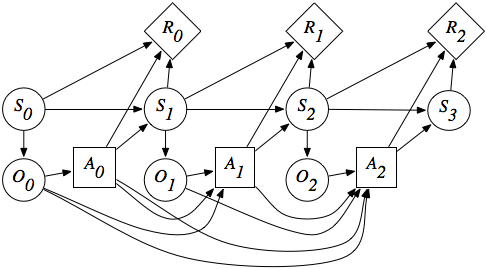
\includegraphics[width=.7\textwidth]{pomdp-dynamic-decision-network.png}
  \caption{The POMDP as a dynamic decision network. \todo[inline]{Replace with
  vector graphics and add initial information $b0$}}
  \label{fig:pomdp}
\end{figure}

In cases where this history can be compressed to a probability for every state
at time $t$, we will refer to this distribution as the \vname{belief},
$b_t(s)$. This belief is a sufficient statistic for optimal decision making.
Consequently, there exists a policy $\pi^*(b_t)$ only dependent on the belief
at the current time step, such that choosing ${a_t=\pi^*(b_t)}$ maximizes
\cref{eq:objective} subject to the constraints on the information pattern
imposed by the \ac{pomdp}, \cite{kaelbling1998planning,
kochenderfer2015decision}. Loosely speaking, $b_t$ preserves all relevant
information contained in the action-observation-history, $h_t$ necessary to
compute the optimal action. The belief is maintained by recursively performing
a Bayesian update,
\begin{equation} \label{eqn:update}
    b'(s') = \frac{\int_{s\in\sspace} \odist(o \mid s, a, s') \tdist(s' \mid s, a) b(s) \, ds}
    {\int_{s'\in\sspace} \int_{s\in\sspace} \odist(o \mid s, a, s') \tdist(s' \mid s, a) b(s) \, ds \, ds'} \text{.}
\end{equation}
with incoming observations, $o$. In the case of a discrete state space,
$\sspace$ integrals a to be replaced with sums. In cases where this update rule
is too complex to be evaluated analytically, Monte Carlo integration may be
used for approximate inference \cite{kochenderfer2015decision,
thrun2005probabilistic}.

Solutions to a \ac{pomdp} are Markov policies on belief states. That is, the
optimal policy $\pi^*(b(s)): \bspace \to \aspace$ selects action ${a =
\pi(b(s))}$ for each belief in the \vname{belief space}, $\bspace$ under the
objective of maximizing \cref{eq:objective}. Alternatively, when thinking of
this procedure in terms of action-observation-histories, the policy may be
envisioned as a conditional plan reasoning over the optimal action to take for
every possible sequence of actions and observations starting from the root
belief, $b_0$. This perspective reveals that the search space of possible
policies rapidly grows with increasing size of $\aspace$ and $\ospace$. In
fact, it has been shown that even in the case of finite-horizon problems
\acp{pomdp} remain PSPACE-complete. Hence, it is reasonable to assume to that
no efficient general algorithm for solving large problems of this class can be
found \cite{papadimitriou1987complexity}. However, recent research has made
significant progress on approximate solution methods, some of which we will use
in this work \cite{silver2010pomcp, somani2013despot, sunberg2018online}.

\section{Online POMDP Solvers}\label{sec:online-pomdp-solvers}

Once a problem has been formalized as a \ac{pomdp}, a wide range of solution
methods can be applied to solve it. On an abstract level, there exist two classes
of solution techniques:

\emph{Offline} methods perform most of the computation prior to execution. That
is, a policy for the entire belief space is computed a priori. At execution
time, actions are selected according to the assignment computed offline.

\emph{Online} methods compute the optimal policy at execution time by planning
from the current belief state. Solution techniques of this kind potentially
leads to redundant computation and more compute per decision step at runtime.
However, in practice they allow to solve much larger \acp{pomdp} since the
reachable belief states are typically a small subset of the full belief space.
By exploiting this local structure online methods allow to compute solutions to
large problems that may be intractable for offline approaches
\cite{kochenderfer2015decision, silver2010pomcp, somani2013despot,
kurniawati2016online}.

In practice, due to the complexity of \acp{pomdp}, even for seemingly simple
problems finding the exact solution is computationally intensive. However,
recent research has put forth online solvers that provide good approximations
to a wide range of problems. This work makes use of two of the most elaborate
state of the art online \ac{pomdp} solvers -- \ac{despot} and \ac{pomcpow}. We
choose these methods since they show superior performance in a wide range of
benchmark problems and outperform other approximate solutions especially for
large \acp{pomdp} \cite{somani2013despot, sunberg2018online}.

In the following subsections we introduce \ac{despot} and \ac{pomcpow} in
greater detail and discuss their theoretical properties.

\subsection{DESPOT}\label{sec:theory-despot}

\begin{algorithm}[htpb]
  \caption{DESPOT \cite{somani2013despot}.}\label{alg:despot}
  \begin{algorithmic}[1]
    \Procedure{Plan}{$b_0$}
      \State $\ell \gets \Call{BuildDespot}{b_0}$
      \State $a^* \gets \max_{a \in \aspace}{\ell(b_0, a)}$
      \If{$L_0(b_0) > \ell(b, a^*)$}
        \State $a^* \gets \pi_0(b_0)$
      \EndIf
      \State \textbf{return} $a^*$
    \EndProcedure\vspace{10pt}

    \Procedure{BuildDespot}{$b_0$}
      \State $\Phib_{b0} \gets K \text{ scenarios sampled from } b_0$
      \State $\mathcal{D} \gets \text{new DESPOT with a single node $b_0$ as the root}$
      \State Initialize $U(b_0), L_0(b_0), \mu(b_0),$ and $\ell(b_0)$ \Comment{TODO: Explain}
      \State $\epsilon(b_0) \gets \mu(b_0) - \ell(b_0)$
      \While{$\epsilon(b_0) > \epsilon_0$ and total running $< T_{\text{max}}$}
        \State $b \gets \Call{Explore}{\mathcal{D}, b}$
        \State $\Call{Backup}{\mathcal{D}, b}$
        \State $\epsilon(b_0) \gets \mu(b_0) - \ell(b_0)$ \Comment{TODO: Think about this}
      \EndWhile
      \State \textbf{return} $\ell$
    \EndProcedure\vspace{10pt}

    \Procedure{Explore}{$\mathcal{D}, b$}
      \While{$\Delta(b) \leq D, E(b) > 0, \text{ and } \Call{Prune}{\mathcal{D}, b} = \text{FALSE}$}
        \If{$b$ is a leaf node in $\mathcal{D}$}
          \State Expand $b$ one level deeper.
          \Statex[3] Insert each new child $b'$ of $b$ into $\mathcal{D}$,
          \Statex[3] and initialize $U(b'), L_0(b'), \mu{(b')}$, and $\ell(b')$.
        \EndIf
        \State $a^* \gets \argmax_{a \in \aspace}{\mu(b, a)}$
        \State $o^* \gets \argmax_{o \in \ospace_{b, a^*}}{E(\tau(b, a^*, z))}$\Comment{Think about this}
        \State $b \gets \tau(b, a^*, z^*)$
      \EndWhile
      \If{$\Delta(b) > D$}
        \State $\Call{MakeDefault}{b}$
      \EndIf
      \State \textbf{return} $b$
    \EndProcedure\vspace{10pt}
  \end{algorithmic}
  \todo[inline]{Figure out how to space this properly.}
  \todo[inline]{Figure out multi column or multi page solution.}
\end{algorithm}

\begin{algorithm}[htpb]
  \begin{algorithmic}[1]
      \Procedure{Prune}{$\mathcal{D}, b$}
        \State \textsc{Blocked} $\gets$ FALSE
        \For{each node $n$ on the path from $b$ to the root of $\mathcal{D}$}
          \If{$n$ is blocked by any ancestor node in $D$}
            \State $\Call{MakeDefault}{n}$
            \State $\Call{Backup}{\mathcal{D}, n}$
            \State \textsc{Blocked} $\gets$ TRUE
          \Else
            \State \textbf{break}
          \EndIf
        \EndFor
        \State \textbf{return} \textsc{Blocked}
      \EndProcedure\vspace{10pt}

      \Procedure{MakeDefault}{$b$}
        \State $U(b) \gets L_0(b)$
        \State $\mu(b) \gets l_0(b)$
        \State $\ell(b) \gets \ell_0(b)$
      \EndProcedure\vspace{10pt}

      \Procedure{Backup}{$\mathcal{D}, b$}
        \For{each node $n$ on the path form $b$ to the root of $D$}
          \State Perform backup on $\mu(x), l(x)$, and $U(x)$.
        \EndFor
      \EndProcedure\vspace{10pt}
  \end{algorithmic}
\end{algorithm}

\todo[inline]{write:}
\begin{itemize}
  \item formal, high-level idea of a DESPOT (idea of scenarios etc.)
  \item the search algorithm on a DESPOT with bounds
  \item explain the difference to POMCPOW (or Monte Carlo methods in general)
  \item point to literature for convergence guarantees
\end{itemize}

\missingfigure{DESPOT tree visualization}

\subsection{POMCPOW}\label{sec:theory-pomcpow}

\acf{pomcpow} is an approximate online \ac{pomdp} solver that combines the idea
of \ac{mcts} -- as utilized in \ac{pomcp} \cite{silver2010pomcp} -- with the
idea of \ac{dpw} \cite{sunberg2018online}.

Before we discuss the algorithmic procedure of \ac{pomcpow} we briefly review
the general idea of \ac{mcts}. This section is thought to be a concise recap of
the fundamental concept and seeks to provide a baseline for understanding how
this technique is adopted in the context of \ac{pomcpow}. A thorough discussion
of \ac{mcts} is beyond the scope of this work. For a detailed survey of
a wide range of \ac{mcts} algorithms, the reader may refer to
\cite{browne2012survey}.

\subsubsection{Monte-Carlo Tree Search}
A theoretically valid solution method for sequential decision making problems
is the construction of the entire policy tree. This tree consists of alternating
layers of states and actions, enumerating all possible future trajectories.
Given this object, extracting the optimal strategy from is trivial. However,
for problems relevant in practice the curse of dimensionality makes simulating
all possible futures intractable.

\acf{mcts} is a method that breaks the curse of dimensionality by utilizing
Monte-Carlo simulations to incrementally construct only important parts of the
policy tree in an asymmetric fashion. As the policy is constructed, the samples
are used to approximate the \vname{state-action value function}, $Q(s, a)$,
also referred to as the \vname{\qfunction}. The approximate \qfunction is used
to focus further exploration of promising parts of the tree, allowing the
algorithm to approximate the optimal policy without attempting the intractable
task of constructing the entire policy tree. This behavior is achieved by
invoking a suitable \emph{tree policy} that balances exploration and
exploitation, the trade-off between looking at new parts of the state-action
space (widening the tree) and further exploring promising trajectories
(deepening the tree). One reason for the popularity of this method is that
it only requires access to a \vname{generative model}, $G$, used to sample new states
given a state-action a pair. That is, no explicit model of the state dynamics is
required, as long as a black box simulator of the environment is available.

To date, \ac{mcts} has been applied to a wide range of problems
\cite{browne2012survey}. While research has put forth many variants of this
algorithm, conceptually they all share the idea of iteratively running
Monte-Carlo simulations until a terminal condition is reached. This terminal
condition may be derived from a convergence criterion, a fixed number of
iterations or a limited computational budget. One iteration of the general
\ac{mcts} algorithm is visualized in \cref{fig:mcts-general}. Each cycle
comprises four steps:

\begin{description}
  \item[Search] The tree policy is invoked to traverse the policy tree
    constructed up to this point. That is, at each state node the tree policy
    selects an action based on the current \qfunction approximation. Once an
    action has been chosen, the next state is selected by sampling from the
    $G$. This search procedure is repeated in an effort to reach
    the most urgent leaf node of the policy tree.
  \item[Expansion] Once an action node is reached that does not have any
    children, a new node is appended to the policy tree by sampling a state
    from $G$ and adding the corresponding actions.
  \item[Rollout] Starting from the newly added node, a reward trajectory is
    simulated by selecting actions according to a \emph{rollout policy}. This
    rollout policy may be as trivial as randomly selecting actions until
    a terminal state is reached or the future cumulative reward becomes
    negligible due to the compounding discount factor. Alternatively, domain
    specific knowledge may be utilized to design a more structured rollout
    strategy. The rollout yields a value estimate for the newly added leaf node.
  \item[Backpropagation] The value estimate obtained from the rollout
    simulation is passed back up the tree to update the \qfunction estimate on
    the path to the root node.
\end{description}

An important factor for the success of of this algorithm is the choice of the
tree policy as this policy must focus the expansion to the relevant part of the
tree. A widely used tree policy is the \ac{uct}. This policy is a greedy policy
with respect to the \vname{upper confidence bound},
\begin{equation}
\label{eqn:ucb} \emph{UCB}(s,a) = Q(s,a) + c \sqrt{\frac{\log N(s)}{N(s,a)}}.
\end{equation}

Here, $N(s, a)$ is the number of times the action node (child) has been
visited, $N(s) = \sum_{a \in \aspace}{N(s, a)}$ is the number of times the
corresponding state node (parent) has been visited, and $c$ is a problem
specific parameter to balance the exploration/exploitation trade-off.
Intuitively, the first term encourages the algorithm to select actions that in
the past showed promising future reward trajectories while the second term
urges the tree policy to expand nodes that have not been sufficiently explored.
For a thorough discussion of convergence properties as well as guidance for the
tuning of $c$, the reader may refer to \cite{kocsis2006bandit, browne2012survey}.

\begin{figure}[htpb]
  \centering
  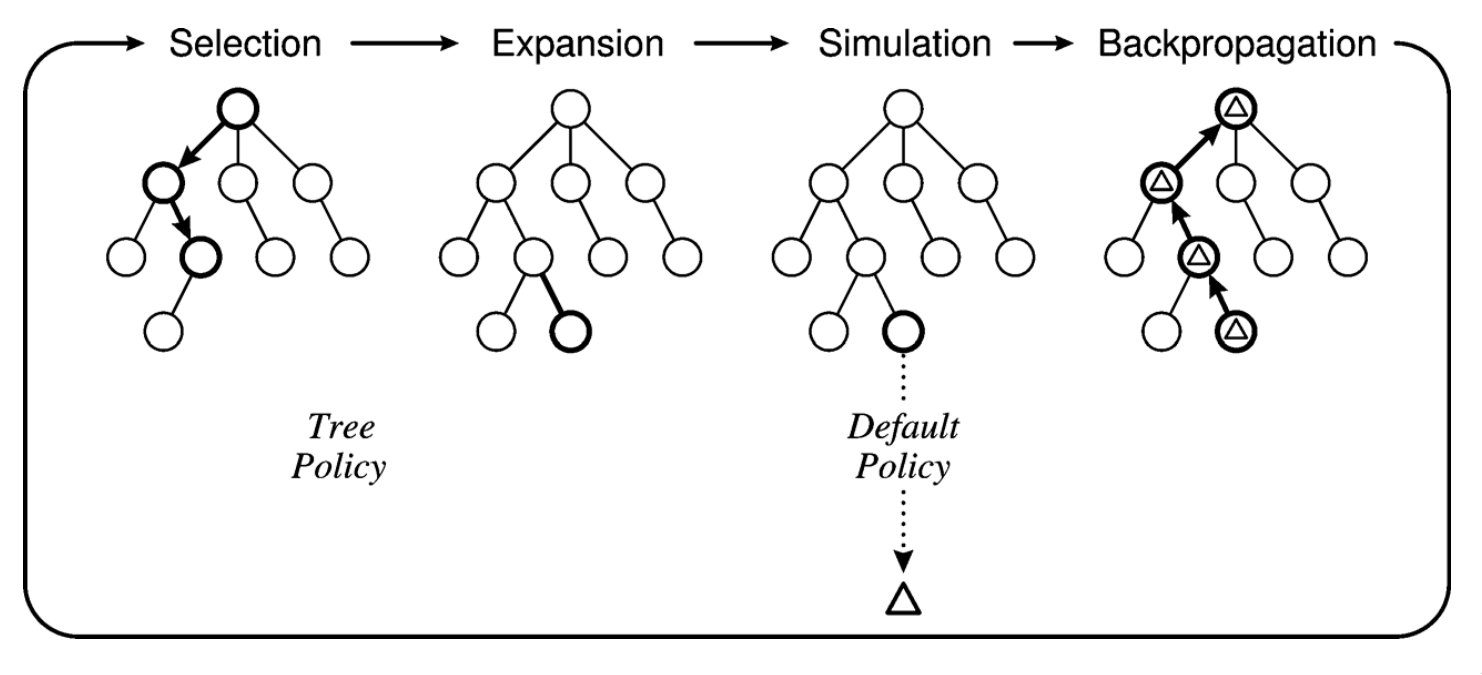
\includegraphics[width=0.8\linewidth]{mcts-general.png}
  \caption{One iteration of the general \ac{mcts} approach
  \cite{browne2012survey}.\todo[inline]{Selection should be called search.
  Simulation should be called Rollout (to be consistent with
  \cite{kochenderfer2015decision}). Draw this in Inkscape.}}
  \label{fig:mcts-general}
\end{figure}

\subsubsection{Double Progressive Widening}

For problems with large or continuous the state and action space, standard
\ac{mcts} as presented in the previous section will produce very shallow trees.
In fact, if the action space is infinite (e.g. continuous or countably
infinite), \ac{mcts} using \ac{uct} will never choose a previously expanded
action at the same state node a second time. This is evident from
\cref{eqn:ucb}. For any unexplored action ($N(s, a) = 0$) the second term is
understood to be unbounded, causing the tree policy to favor untried actions.
Additionally, if the state space is continuous and the transition probability
density is finite, the event of $G$ generating the same state twice has
probability zero. As a result, simulated trajectories will never pass through
the same state node, causing the policy tree to never expand beyond the first
layer.

Progressive widening addresses this issue by artificially limiting the number
for children of a node to $kN^\alpha$, where $N$ is the number of times the
parent has been visited and $k$ and $\alpha$ are problem specific tuning
parameters \cite{couetoux2011continuous}. Originally, this strategy has been
applied to the action space, as described in \cref{alg:aprogwiden}. \acf{dpw}
extends this idea to additionally apply to $\sspace$. In either case, if the
number of children at a node exceeds the progressively incremented limit
(\cref{alg:aprogwiden:lin:check}), instead of generating a new child, one of
the previously generated nodes is selected. By this means, \ac{mcts} expands to
deeper layers earlier and widens the tree as additional iterations are run.
This results in less myopic policies for problems with large state and action
spaces \cite{couetoux2011continuous}.

\begin{algorithm}
  \caption{Progressive widening applied to $\aspace$ \cite{sunberg2018online}.}\label{alg:aprogwiden}
  \begin{algorithmic}[1]
      \Procedure {ActionProgWiden}{$h$}
          \If{$|C(h)| \leq k_a N(h)^{\alpha_a}$}\label{alg:aprogwiden:lin:check}
              \State $a \gets \Call{NextAction}{h}$
              \State $C(h) \gets C(h) \cup \{a\}$
          \EndIf
          \State $\textbf{return } \underset{a \in C(h)}{\argmax}\, Q(ha) + c \sqrt{\frac{\log N(h)}{N(ha)}}$
      \EndProcedure\vspace{10pt}
  \end{algorithmic}
\end{algorithm}

\subsubsection{POMCPOW Algorithm}

The algorithmic procedure for \ac{pomcpow} fundamentally resembles the idea of
\ac{mcts} with a set of modifications for application in the \ac{pomdp} domain.
Instead of reasoning over state-action sequences, the policy tree spans over
action-observation trajectories starting from the initial belief, $b_0$. In
contrast to \ac{pomcp}, \ac{pomcpow} uses \ac{dpw} to focus search on
a progressively expanded set of actions and observations \cite{silver2010pomcp,
sunberg2018online}. This enhancement allows to yield deeper and more richly
sampled policy trees even in the case of large action and observation spaces.
Finally, since \ac{dpw} constraints the set of considered observations, the
algorithm uses a weighted particle collection to represent the outcome
statistics at observation nodes. By this means, the outcome of the generative
model can be fixed to fall inside the allowed set to avoid sample rejection,
while the weighted belief update prevents an erroneous distribution shift.

A detailed pseudo code representation of the algorithmic procedure is provided
in \cref{alg:pomcpow}. With the preceding introduction of \ac{mcts} and the
aforementioned outline of the algorithms key ideas in mind, we proceed by
discussing each subroutine in greater detail.

In addition to the variables defined in the previous sections, we introduce the
following notation to describe the \ac{pomcpow} algorithm: $h$ represents
a history, ($b_0$, $a_1$, $o_1$, $a_2$, \dots, $a_k$, $o_k$), as introduced in
\cref{sec:pomdp}, $ha$ and $hao$ are shorthand for concatenation of $h$ with
$a$ or $(a, o)$, respectively. $d$ denotes the remaining depth to explore, with
$d_\text{max}$ the maximum depth; $C(h)$ is the list of children of node $h$;
$N(h)$ denotes the number of visits of node $h$; $M(hao)$ is a count for the
number of times the observation terminated history $hao$ has been sampled by
the generative model, $G$. $B(h)$ represents a list of states associated with
node $h$, with $W(h)$ the corresponding weights.

\textbf{Plan}\\
The \textsc{Plan} procedure represents the outer loop of the algorithm. Input
to the function is the current belief, $b$, as obtained from a belief updater.
Typically, $b$ is the output of a particle filter. Starting at $b$, the
algorithm performs $n$ iterations of \ac{mcts} to obtain a local approximation
the action value function, $Q$. The procedure is parametrized with
$d_\text{max}$, the maximum search depth of the policy tree. Finally, the planner
selects the action, that maximizes the obtain \qfunction approximation.

\textbf{Simulate}\\
The \textsc{Simulate} procedure resembles a recursive implementation of
a single \ac{mcts} iteration. Inputs to the function are a sampled state, $s$,
an action-observation history as introduced in \cref{sec:pomdp}, $h$, as well
as the remaining search depth, $d$. Unless the maximum depth is reached, the
algorithm proceeds by selecting an action $a$ using action progressive
widening. Given this action, a state-observation-reward tuple is sampled from
the generative model. Subsequently, observation progressive widening
(\crefrange{alg:lin:oprogwide_start}{alg:lin:oprogwide_end}) is applied to
either generate a new observation and increment the corresponding counter, or
sample one of the previously generated observations, $o \in C(ha)$. The
generated state, $s'$, is added to the state list at the observation node,
$B(hao)$. In order to resemble a weighted particle belief, the corresponding
weight is chosen according to the observation model, $\odist(o \mid s, a, s')$,
and is stored in the associated weight vector, $W(hao)$.

If the observation is not a child of this action terminated history node, a new
observation node is created and a rollout in the spirit of \ac{mcts} is
performed. Otherwise, search on the partially constructed policy tree continues
one level deeper by sampling a state, $s'$, from the weighted particle
collection to proceed with the next \textsc{Simulate} recursion.

Finally, backpropagation is performed by passing the simulated \vname{total}
reward up the recursion stack and updating the \qfunction approximation
accordingly.

\begin{algorithm}[H]
    \caption{POMCPOW \cite{sunberg2018online}.}\label{alg:pomcpow}
    \begin{algorithmic}[1]
        \Procedure{Plan}{$b$}
            \For{$i \in 1:n$}
                \State $s \gets \text{sample from }b$
                \State $\Call{Simulate}{s, b, d_\text{max}}$
            \EndFor
            \State $\textbf{return } \underset{a}{\argmax}\, Q(ba)$
        \EndProcedure\vspace{10pt}

        \Procedure {Simulate}{$s$, $h$, $d$}
            \If{$d = 0$}
                \State \textbf{return} $0$
            \EndIf
            \State $a \gets \Call{ActionProgWiden}{h}$
            \State $s',o,r \gets G(s,a)$
            \If{$|C(ha)| \leq k_o N(ha)^{\alpha_o}$}\label{alg:lin:oprogwide_start}
                \State $M(hao) \gets M(hao) + 1$
            \Else
                \State $o \gets \text{select } o \in C(ha) \text{ w.p. } \frac{M(hao)}{\sum_{o} M(hao)}$
            \EndIf\label{alg:lin:oprogwide_end}
            \State $\text{append } s' \text{ to } B(hao)$ \label{lin:insert}

            \State $\text{append } \odist(o \mid s, a, s') \text{ to } W(hao)$ \label{lin:weight}
            \If{$o \notin C(ha)$}
                \State $C(ha) \gets C(ha) \cup \{o\}$
                \State $total \gets r + \gamma \Call{Rollout}{s', hao, d-1}$
            \Else
                \State $s' \gets \text{select } B(hao)[i] \text{ w.p. } \frac{W(hao)[i]}{\sum_{j=1}^m W(hao)[j]}$ \label{lin:sample}
                \State $r \gets \reward(s,a,s')$
                \State $total \gets r + \gamma \Call{Simulate}{s', hao, d-1}$
            \EndIf
            \State $N(h) \gets N(h)+1$
            \State $N(ha) \gets N(ha)+1$
            \State $Q(ha) \gets Q(ha) + \frac{total - Q(ha)}{N(ha)}$
            \State \textbf{return} $total$
        \EndProcedure\vspace{10pt}
    \end{algorithmic}
\end{algorithm}

\missingfigure{graphical model of POMCPOW-Tree with weighted scenarios.}

\section{Tools and Software Framework}

Solving a \ac{pomdp} poses a challenging problem from both, the
implementational\todo{is this the right phrasing?} and computational
perspective. Therefore, suitable software tooling is required that provides
a simple but expressive way of describing problems and solvers while leveraging
the full computational power of the hardware involved.

This section briefly discusses the tooling choices made for the experiments
conducted throughout this work. This discussion is not thought to be a detailed
comparison of \ac{pomdp} frameworks but rather seeks to provide insight into
how the tools used here can help to accelerate the solution process.

To date, there exist a number of frameworks that are capable of solving
sequential decision making problems under uncertainty, some of which also
accommodate partially observable domains. In this work we make use of the novel
framework \pomdpsjl, an open-source interface for solving \acp{mdp} and
\acp{pomdp} \cite{egorov2017pomdps}. Unlike other popular frameworks like APPL
(\cite{appl}), AI-Toolbox (\cite{aitoolbox}), and ZMDP (\cite{zmdp}), \pomdpsjl
is not written in \emph{C++} but in the \emph{Julia} programming language. This
enables the user to flexibly build prototypes while the high-performance nature
of the language allows to scale ideas to run extensive simulations on large
multi-node clusters. Benchmarks in the past have shown that despite being
a high-level language that abstracts a lot of complexity, the execution time of
code written in \emph{Julia} can still compete with \emph{C++} implementations.
In fact, experiments we ran to evaluate the runtime for one of the problems
studied in \cref{chap:hri} suggest that the highly-optimized code produced by
the \emph{Julia} compiler may even outperform a \emph{C++} implementation,
unless the later is carefully tuned by an experienced software engineer. The
results of this problem specific benchmark can be found in \todo{point to
appendix}.

In addition to the advantages generated by the choice of programming language,
\pomdpsjl provides a simple yet expressive interface to describe, solve and
simulate \acp{pomdp}. The toolbox specifies abstract interfaces for three
conceptual elements: \emph{problems}, \emph{solvers} and \emph{experiments}.
This design decouples these subdomains, thus ensuring that code can be written
for each of them separately while not sacrificing interchangeability. Finally,
the associated \emph{JuliaPOMDP} community provides a number of
state-of-the-art \ac{mdp} and \ac{pomdp} solvers as well as a rich library of
tools for implementing and evaluating solvers and solutions.
